\chapter{基于马尔可夫链和Perron–Frobenius算法用于分布式电力系统经济调度的过渡矩阵Q优化}
\label{cha:Algorithm}

\section{概述}

本章基于马尔可夫链和Perron–Frobenius算法\cite{yan2019consensus}阐述一种新的用于分布式电力系统经济调度的过渡矩阵Q优化方法,提出了一套完整的分布式ED问题的物理和数学模型,实现了尽可能快的迭代。构建了分布式通信协议,并证明了迭代结束时一定可以得到的是帕累托最优。最后通过一个算例说明了共识达到的具体方法。

\section{分布式经济调度模型}

\subsection{物理模型}

现阶段研究的物理模型公式如式~\ref{eq:phymodel},其中,N是机组数量,$p_{i}$是机组出力,$W_{i}\left(p_{i}\right)$是机组出力成本函数,$\lambda_{i}\left(p_{i}\right)$是边际成本函数,$\alpha_{i}$ $\beta_{i}$ $\gamma_{i}$ 是发电机组出力成本函数中的参数,其中$\alpha_{i}$是机组的假想最低成本,$\beta_{i}$是边际成本关于机组出力边际增长率的倒数,可称是“出力-价格灵敏度”,$\gamma_{i}$是线性外推得到的零边际成本下假想机组出力。$L_{i}$是节点i处的负荷。$\underline{p}_{i}$和$\bar{p}_{i}$分别是机组出力上限与下限。

\begin{equation}
    \begin{aligned}
    &\min W(\mathbf{P})=\sum_{i=1}^{N} W_{i}\left(p_{i}\right)\\
    &\sum_{i=1}^{N} p_{i}=\sum_{i=1}^{N} L_{i}\\
    &\underline{p}_{i} \leq p_{i} \leq \bar{p}_{i}, \forall i\\
    &W_{i}\left(p_{i}\right)=\frac{\left(p_{i}-\alpha_{i}\right)^{2}}{2 \beta_{i}}+\gamma_{i}, i=1,2, \ldots, N\\
    &\lambda_{i}\left(p_{i}\right)=\frac{\partial W_{i}\left(p_{i}\right)}{\partial p_{i}}=\frac{1}{\beta_{i}}\left(p_{i}-\alpha_{i}\right), i=1,2, \ldots, N\\
    &p_{i}=\beta_{i} \lambda_{i}+\alpha_{i}
    \end{aligned}
    \label{eq:phymodel} 
\end{equation}

在边际成本函数的基础上,目标函数等价于求价格共识$\lambda$,其含义是:

\begin{itemize}
    \item 各节点处都有边际成本$\lambda_{i}$,必须保证全部$\lambda_{i}$相等或足够接近。
    \item 在$\lambda_{i}$下,由式~\ref{eq:phymodel}-6决定的机组出力$p_{i}$必须满足全部约束条件。
\end{itemize}

\subsection{数学模型-有向图邻接矩阵}

% 在图论中,\textbf{图}(Graph)用于表示物件与物件之间的关系,是图论的基本研究对象。一张图由一些小圆点(称为\textbf{顶点}或\textbf{结点})和连结这些圆点的直线或曲线(称为\textbf{边})组成。

% 如果给图的每条边规定一个方向,那么得到的图称为有向图,其边也称为有向边。在有向图中,与一个节点相关联的边有出边和入边之分,而与一个有向边关联的两个点也有始点和终点之分。相反,边没有方向的图称为无向图。

% 对有向图而言,顶点的度还可分为出度和入度。一个顶点的出度(Out-degree)为i,是指有i条边以该顶点为起点,或说与该点关联的出边共有i条。入度的概念也类似。

在图论和计算机科学中,邻接矩阵是用于表示有限图的方阵。矩阵的元素指示图中的顶点对是否相邻。

对于顶点集为V的简单图,邻接矩阵为| V | ×| V | 矩阵A使得当存在从顶点i到顶点j的边时元素$A_{ij}$为1,当没有边时为零。矩阵的对角元素全为零,因为在简单图中不允许从顶点到自身的边缘(循环)。在代数图论中有时用代数变量代替非零元素也很有用。

通过将每个两个顶点之间的边数存储在相应的矩阵元素中,并允许非零对角元素,可以将相同的概念扩展到带循环的多重图和图形。只要遵循一致的约定,就可以将循环计数一次(作为单个边)或两次(作为两个顶点边的入射)。无向图通常使用计数循环次数的后一种约定,而有向图通常使用前一种约定。

在有向图中,可以通过对相应列的条目求和来计算顶点的入度,而可以通过对相应行的条目求和来计算顶点的出度。

\begin{figure}[htbp]
    \begin{minipage}{0.48\textwidth}
      \centering
      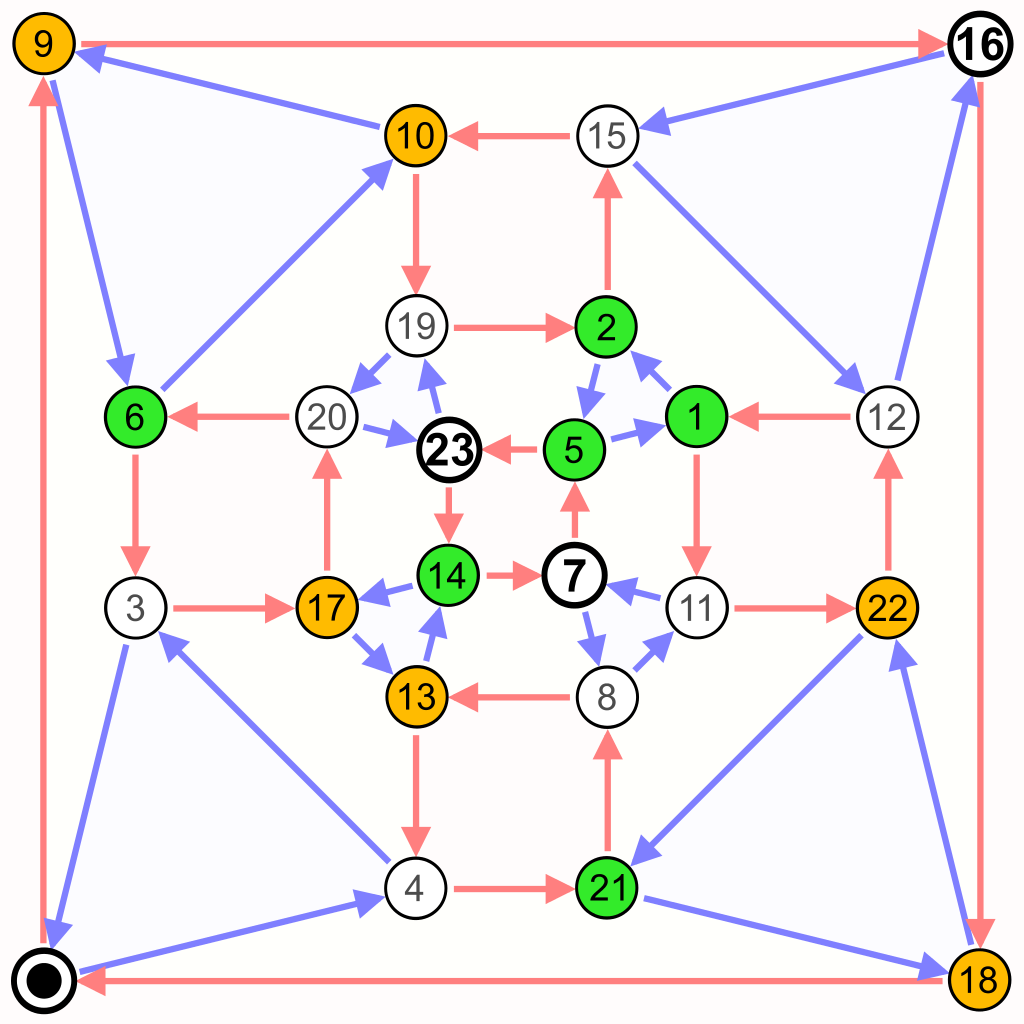
\includegraphics[height=7cm]{numbers.png}
      \caption{Cayley有向图}
      \label{fig:Directed-Cayley-graph}
    \end{minipage}\hfill
    \begin{minipage}{0.48\textwidth}
      \centering
      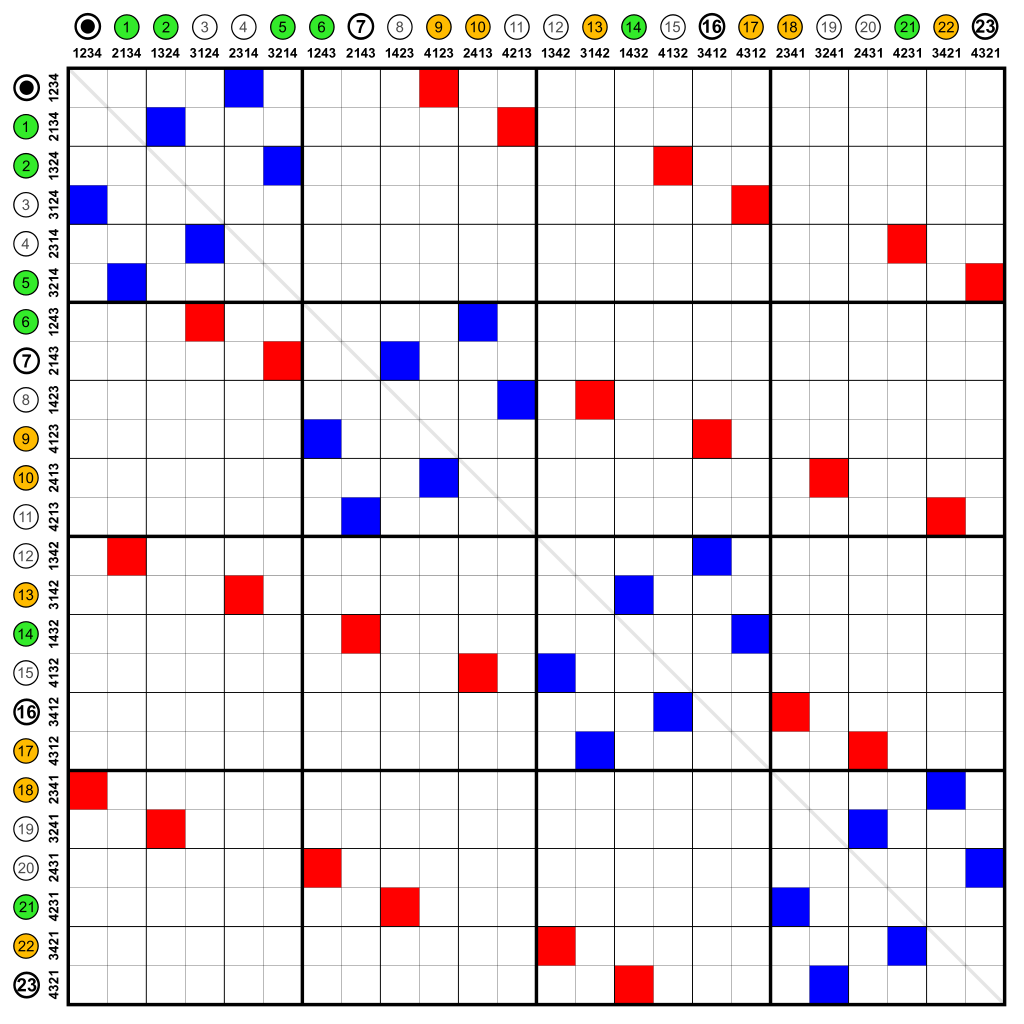
\includegraphics[height=7cm]{adjacency_matrix.png}
      \caption{邻接矩阵}
      \label{fig:Adjacency-matrix}
    \end{minipage}
\end{figure}

\subsection{链式通信协议}
对于一个强连通的电网,我们使用有向图的邻接矩阵A来描述其通信拓扑:

\begin{equation}
    \mathbf{A}=\left[a_{i j}\right]_{N \times N}
\end{equation}

\begin{equation}
    a_{i j}=\left\{\begin{array}{l}
    {1} \\
    {0}
    \end{array}\right.
\end{equation}

其中,1表示通信节点j能向i发送消息并被i接收。

链式通信协议迭代更新每个节点的状态变量如下:

\begin{equation}
    s_{i}^{(k+1)}=\sum_{j=1}^{N} q_{i j} s_{j}^{(k)}, i=1,2, \ldots, N
\end{equation}

矩阵形式为:

\begin{equation}
    \mathbf{s}^{(k+1)}=\mathbf{Q} \mathbf{s}^{(k)}
\end{equation}

由于在电网中,下一轮迭代的状态变量仅和上一轮迭代的状态变量相关,具有无记忆性。参考Markov chain可得,Q为过渡矩阵,有每一次迭代时有向图的边的权重信息。

在实际物理层中,我们选取状态变量为

\begin{equation}
    s_{i}^{(k)}=p_{i}^{(k)}-\alpha_{i}
\end{equation}

其中,$p_{i}^{(k)}$是第k轮迭代的机组i的出力,$\alpha_{i}$为线性外推得到的零边际成本下的假想机组出力。 $s_{i}^{(k)}$是机组i的溢价出力量,这部分出力将抬高机组的边际成本$\lambda_{i}$。

链式通信协议物理含义为:每一回合,每台机组将自身出力按特定比例转移给相邻节点。

\section{过渡矩阵优化}

由Perron–Frobenius定理可知:过渡矩阵的次大特征值$\sigma_{2}$决定链式通信协议收敛速率,主特征向量$\sigma_{1}$(Perron向量)决定链式通信协议的最终收敛结果。因此引入F-范数$\|\mathbf{Q}\|_{F}$优化过渡矩阵,实现机组出力的合理分配,提高收敛速度。

\subsection{F-范数调整过渡矩阵Q的元素值}

% 使用特定的矩阵范数(matrix norm,模)来简化之后的迭代运算,这里采用弗罗贝尼乌斯范数(Frobenius norm)或称希尔伯特-施密特范数(Hilbert–Schmidt norm),这个范数可用不同的方式定义:

使用Frobenius norm来简化之后的迭代运算,定义:

\begin{equation}
    \|A\|_{F}=\sqrt{\sum_{i=1}^{m} \sum_{j=1}^{n}\left|a_{i j}\right|^{2}}=\sqrt{\operatorname{trace}\left(A^{*} A\right)}=\sqrt{\sum_{i=1}^{\min \{m, n\}} \sigma_{i}^{2}}
\end{equation}

这里$A^*$表示$A$的共轭转置,$σ_i$是$A$的奇异值(特征值)

% 这里A*表示A的共轭转置,σi是A的奇异值(特征值),并使用了迹函数。弗罗贝尼乌斯范数与Kn上欧几里得范数非常类似,来自所有矩阵的空间上一个内积。

% 弗罗贝尼乌斯范数是服从乘法的且在数值线性代数中非常有用。这个范数通常比诱导范数容易计算。

在这里有:

\begin{equation}
    \|\mathbf{Q}\|_{F}=\sqrt{\sum_{i=1}^{N} \sum_{j=1}^{N}\left|q_{i j}\right|^{2}}
\end{equation}

\begin{equation}
    \|\mathbf{Q}\|_{F} \geq \sqrt{\sum_{i=1}^{N}\left|\sigma_{i}\right|^{2}}
\end{equation}

\begin{equation}
    1=\left|\sigma_{1}\right| \geq\left|\sigma_{2}\right| \geq \ldots \geq\left|\sigma_{N}\right|
\end{equation}

优化目标函数:

\begin{equation}
    \min \|\mathbf{Q}\|_{F}^{2}=\sum_{i=1}^{N} \sum_{j=1}^{N}\left|q_{i j}\right|
\end{equation}

优化目标函数物理意义:最小化F范数,相当于最小化次大特征值,优化收敛速率

\subsection{过渡矩阵Q的约束}

过渡矩阵Q满足以下约束条件:

\begin{equation}
    \mathbf{Q}=\left[q_{i j}\right]_{N \times N}
\end{equation}

\begin{equation}
    q_{i j}\left\{\begin{array}{l}
    {\geq 0} \\
    {=0}
    \end{array}\right.
\end{equation}

当节点j不能向节点i发送信息时为0

还需要保证总出力不变:

\begin{equation}
    \mathbf{Q} \mathbf{1}^{T}=\mathbf{1}^{T}
\end{equation}

即:

\begin{equation}
    \sum_{j=1}^{N} q_{i j}=1, i=1,2, \ldots, N
\end{equation}

为使得链式通信协议收敛于过渡矩阵Q,需保证过渡矩阵的Perron向量恰好等于出力-价格灵敏度向量$\boldsymbol{\beta}=\left[\beta_{1}, \beta_{2}, \ldots, \beta_{N}\right]^{T}$,即保证出力比稳定为$\boldsymbol{\beta}_{1}: \boldsymbol{\beta}_{2} \ldots$。其中$\lambda_{i}=p_{i} / \beta_{i}$,即机组i的成本微增率与出力成正比,$\boldsymbol{\beta}$为出力/价格比例系数。

\begin{equation}
    \mathbf{Q} \boldsymbol{\beta}=\boldsymbol{\beta}
\end{equation}

即:

\begin{equation}
    \sum_{j=1}^{N} q_{i j} \beta_{j}=\beta_{i}, i=1,2, \ldots, N
\end{equation}

\subsection{过渡矩阵优化求解}

即求解以下二次规划问题:

\begin{equation}
    \begin{aligned}
    &\min _{q_{y}}\|\mathbf{Q}\|_{F}^{2}=\sum_{j=1}^{N} \sum_{i=1}^{N}\left|q_{i j}\right|^{2}\\
    &\text { s.t. } \quad q_{i j}\left\{\begin{array}{ll}
    {\geq 0} & {\quad a_{i j}=1} \\
    {=0} & {\quad a_{i j}=0}
    \end{array}\right.\\
    &\mathbf{Q} \mathbf{1}^{T}=\mathbf{1}^{T}\\
    &\mathbf{Q} \boldsymbol{\beta}=\boldsymbol{\beta}
    \end{aligned}
\end{equation}

一般二次规划问题求解形式为:

\begin{equation}
    \begin{aligned}
    &\min \mathbf{x}^{T} \mathbf{x}\\
    &\text { s.t. } \quad \mathbf{A}_{1} \mathbf{x}=\mathbf{b}_{1}
    \end{aligned}
\end{equation}

其中x的每一个元素即是过渡矩阵Q的一个非零元素。该二次规划问题的优化解为:

\begin{equation}
    \mathbf{x}^{*}=\mathbf{A}_{1}^{T}\left(\mathbf{A}_{1} \mathbf{A}_{1}^{T}\right)^{-1} \mathbf{b}_{1}
\end{equation}

将x*的每个元素的值还原到过渡矩阵Q的相应位置上,可得到经优化的过渡阵。

\section{分布式ED协议的实现方式}

每个节点独立算出$\beta_{i}$出力/价格比例系数,

出力-价格灵敏度向量$\boldsymbol{\beta}$与邻接矩阵$\boldsymbol{A}$结合,得出优化后的过渡矩阵$\boldsymbol{Q}$

根据过渡矩阵与链式通信拓扑有向图权重的对应关系,的第j列元素代表始端节点与机组j的边的权重。因此把过渡矩阵$\boldsymbol{Q}$按列拆分,将第j列元素发送给机组j的节点。

节点i独立算出其初始溢价出力量$s_{i}^{(0)}=L_{i}-\alpha_{i}$

按过渡矩阵Q,迭代运行链式通信协议。

\begin{equation}
    s_{i}^{(k+1)}=\sum_{j=1}^{N} q_{i j} s_{j}^{(k)}, i=1,2, \ldots, N
\end{equation}

节点j计算出$q_{i j} s_{j}^{(k)}, i=1,2, \ldots, N$,并分别将$q_{i j} s_{j}^{(k)}$发给节点i。(若$A_{i j}$为0,则此项为0,不影响其他节点)

k次迭代后,节点i的出力和电价为:

\begin{equation}
    \begin{aligned}
    &p_{i}^{(k)}=s_{i}^{(k)}+\alpha_{i}\\
    &\lambda_{i}^{(k)}=s_{i}^{(k)} / \beta_{i}
    \end{aligned}
\end{equation}

当迭代过程中式~\ref{eq:delta}条件满足,则价格达成共识,可以执行目前的定价。

\begin{equation}
    \left|\lambda_{i}^{(k+1)}-\lambda_{i}^{(k)}\right|<\delta
    \label{eq:delta}    
\end{equation}

其中$\delta$为误差容限,表示电价求解精度。

\section{迭代结束将得到帕雷托最优的证明}

本节证明迭代结束时各节点出力达到帕雷托最优(Pareto Optimality),即在误差允许的范围内ED最优解。

\begin{equation}
    \mathbf{1}^{T} \mathbf{s}^{(k+1)}=\mathbf{1}^{T} \mathbf{Q} \mathbf{s}^{(k)}=\mathbf{1}^{T} \mathbf{s}^{(k)}=\mathbf{1}^{T} \mathbf{s}^{(0)}=\sum_{i=1}^{N}\left(L_{i}-\alpha_{i}\right)
\end{equation}

由于终止时各变量趋于稳定,由Perron-由Perron–Frobenius定理:

\begin{equation}
    \mathbf{s}^{(k)}=r \boldsymbol{\beta}
\end{equation}

得:

\begin{equation}
    r=\sum_{i=1}^{N}\left(L_{i}-\alpha_{i}\right) / \sum_{i=1}^{N} \beta_{i}=\lambda_{i}^{(k)}
\end{equation}

表明达到价格共识,并满足功率平衡约束:

\begin{equation}
    \sum_{i=1}^{N}\left(\beta_{i} \lambda_{i}^{(k)}+\alpha_{i}\right)=\sum_{i=1}^{N} L_{i}
\end{equation}

\section{考虑每个节点出力上下限的处理}

当某节点的出力超上下限时,可用虚拟功率法调整出力分配。

\begin{equation}
    S_{i}^{(k+1)}=\left(\sum_{j=1}^{n} q_{i j}\left(s_{j}^{(k)}+\Delta p_{j}^{(k)}\right)\right)-\Delta p_{i}^{(k)}
\end{equation}

\begin{equation}
    \Delta p_{i}^{(k+1)}=\max \left\{\Delta p_{i}^{(k)}+r_{i}^{(k)}\left(s_{i}^{(k)}+\alpha-\bar{p}_{i}\right), 0\right\}
\end{equation}

k能被t整除时为1,反之为0:

\begin{equation}
    r_{i}^{(k)}=\left\{\begin{array}{l}
    {1} \\
    {0}
    \end{array}\right.
\end{equation}


终止条件增加一条:$\Delta p_{i}^{(k)}=0$

$\Delta p_{i}^{(k)}$为机组i引进的虚拟功率,取值为非负数。当机组i的出力到达上限时,由于向外发送了出力,导致整个系统价格抬高。
